\documentclass[a4paper,12pt]{article}

\usepackage{graphicx}
\usepackage[utf8]{inputenc}
\usepackage[T1]{fontenc}
\usepackage{amsmath}
\usepackage{caption}
\usepackage{subcaption}

\title{ Mecânica Clássica I \\ Coordenadas - Esféricas}
\author{}
\date{}
\begin{document}
	\maketitle
	\paragraph \indent A maior diferença entre coordenadas esféricas e cartesianas é visualizar que os versores $\hat{r}, \hat{\theta}, \hat{\varphi}$ variam com o tempo, não é tão difícil de entender, porém nem sempre fica claro o que essa dependência significa.
	
	\paragraph \indent Não faz sentido falar em angulos $\theta$ ou $\phi$ se estivermos descrevendo apenas a posição de um ponto no espaço em relação a origem (Figura 1a) , só existem angulos quando temos mais de um ponto no espaço além da origem, definindo assim o eixo polar (Figura 1b) e um plano no espaço, por fim, para completar todo o espaço tri-dimensional devemos considerar também um segundo eixo, eixo azimutal (Figura 1c) ortogonal ao plano já definido.
	\\
	\begin{figure}
		\centering
		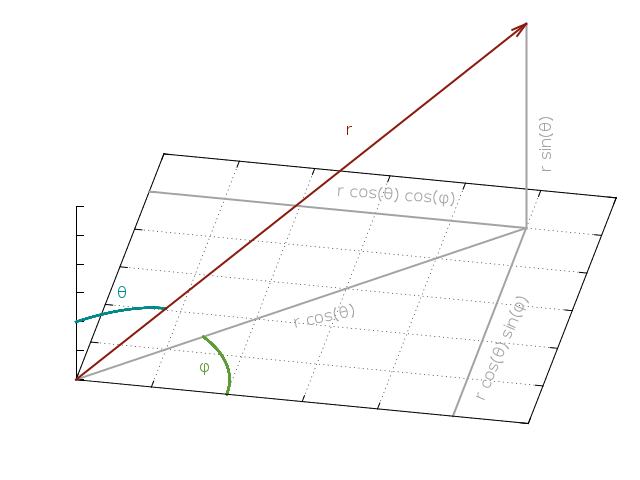
\includegraphics[scale=0.3]{SphericalCoordinates.png}
	\end{figure}
		
	\paragraph \indent Diferente das coordenadas cartesianas em que os eixos $\hat{i},\hat{j},\hat{k}$ são fixos. Neste sistema $\hat{r},\hat{\theta}.\hat{\varphi}$ variam com o tempo. de modo que:
	 
	\begin{equation*}
	\begin{cases}
		x = r sin(\theta) cos(\varphi)  &\\
		y = r sin(\theta) sin(\varphi) &\\
		z = r cos(\theta) &
	\end{cases}
	\end{equation*}
	
	\paragraph \indent Tente visualizar o vetor $\vec{\theta}$ em um movimento circular uniforme como na e note que em cada instante de tempo ele terá uma posição diferente se olhado no espaço cartesiano.

	Velocidade radial: velocidade com que o objeto se aproxima ou se afasta da origem na direção radial.
Velocidade tangencial: é perpendicular a r^ sendo orientada na direçoe azimutal ou polar
Velocidade angular: descreve a variação angular nas direções polar ou azimutal.
Aceleração centripeta:, característico de movimentos curvilíneos ou circulares. Ela é perpendicular à velocidade e aponta para o centro da trajetória.
Aceleração angular: é a variação da velocidade angular no tempo
Aceleração de Coriolis: Aceleração de um corpo que se move em relação a um sistema de referência, medida em outro sistema de referência que apresenta uma aceleração angular em relação ao primeiro.
Sugestão de site para a visualização em 3D: http://www.igm.mat.br/aplicativos/index.php?option=com_content&view=article&id=286:coord
	\[  \]
	 

\end{document}
